\documentclass[12pt,a4paper]{article} 
\usepackage[utf8]{inputenx} 
\usepackage[spanish]{babel} 
\usepackage[left=2cm,right=2cm,top=2cm,bottom=2cm]{geometry}
\usepackage{scrextend}
\usepackage{marvosym}
\usepackage{pifont} % Generación de símbolos especiales
\usepackage{textcomp}
\usepackage{newpxtext}
\usepackage{newpxmath}
\usepackage[T1]{fontenc} % Codificación de salida    
\usepackage{microtype} % Mejoras de microtipografía en la obtención de PDF (sólo para pdflatex)
\usepackage[hyphens]{url} % Para escritura de URL
\urlstyle{sf} % Estilo de URL sin serifas para que tengan un mejor aspecto

% Paquetes para obtener un mayor control de las listas
\usepackage{paralist} % Mayor control de listas
\usepackage{multicol} % Elementos en varias columnas
\usepackage[breaklinks]{hyperref}
\usepackage{graphicx}
\usepackage{caption}
\captionsetup[figure]{labelformat=empty}
\author{Javier Monescillo Buitrón \and Iván Illán Barraya \and Alejandro Medina Jiménez \and Julián García Sánchez}
\title{Implementación de un procesador de lenguajes para Autómatas de Moore}
\date{\today}
%%%%%%%%%%%%%%

\begin{document}
	
	\maketitle
	
	\begin{figure}[h]
		\centering
		
\includegraphics[width=0.25
		\linewidth]{image004}
		\caption{}
		\label{fig:image004}
	\end{figure}

	\newpage
	\tableofcontents
	\newpage
	
	\section{¿Qué es un autómata de Moore?}
	En Teoría de la computación una \textbf{Máquina de Moore} es un autómata de estados finitos para el cual la salida en un momento dado sólo depende de su estado en ese momento, mientras la transición al siguiente estado depende del estado en que se encuentre y de la entrada introducida.
	El diagrama de estados para una máquina de Moore incluirá una señal de salida para cada estado.
	
	\begin{figure}[h]
		\centering
		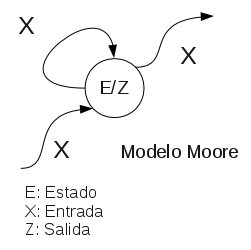
\includegraphics[width=0.5\linewidth]{Modelo-moore}
		\caption{Ejemplo de Máquina de Moore simple}
		\label{fig:modelo-moore}
	\end{figure}
	
	
	
	El nombre de \textbf{Máquina de Moore} viene de su promotor Edward F. Moore, un pionero de las máquinas de estados, quien escribió \textit{Gedanken-experiments on Sequential Machines,} pp 129-153, Estudios de Autómatas, Anuales de los Estudios Matemáticos, no. 34, Princenton Universityy Press, Princenton, N.J., 1956.
	
	\subsection{Definición formal}
	Una máquina de Moore se define como una 6-tupla:
	\[ Mmor = (S,S_{0},\Sigma,\Lambda,T,G)  \]
	donde definimos los siguientes elementos:
	\begin{itemize}
		\item S: es un conjunto finito de estados
		\item $S_{0}$: es el estado inicial
		\item $\Sigma$: alfabeto de entrada
		\item $\Lambda$: alfabeto de salida
		\item $T$ : funcion transicion
		\item $G$ funcion transicion salida
	\end{itemize}
	\clearpage

	\subsection{Ejemplo concreto}
	Definimos una Máquina de Moore para regular el tráfico en el siguiente cruce con los siguientes semáforos:
		
	\begin{figure}[h]
		\centering
		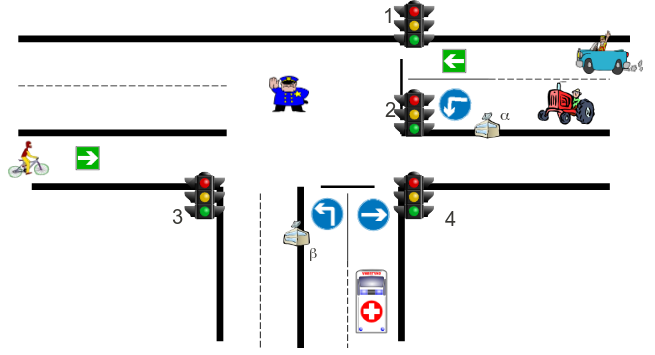
\includegraphics[width=0.4\linewidth]{4}
		\caption{}
		\label{fig:4}
	\end{figure}

El alfabeto de entrada $\Sigma$: {(0,0),(0,1),(1,0),(1,1)}

	\begin{itemize}
		\item (a,b), donde a es el estado para el sensor $\alpha$ y b para el sensor $\beta$
		\item 0 indica que no hay coches en la cola
		\item 1 indica que hay coches en la cola
	\end{itemize}

El alfabeto de salida $\Lambda$: { ($a_{1},a_{2},a_{3},a_{4},a_{i}\epsilon$ (A,V,R) )
	\begin{itemize}
		\item $a_{1}$ es el estado del semáforo 1
		\item $a_{2}$ es el estado del semáforo 2
		\item $a_{3}$ es el estado del semáforo 2
		\item $a_{4}$ es el estado del semáforo 2
	\end{itemize}

	\begin{center}
		El diagrama de estados sería el siguiente:
	\end{center}

	\begin{figure}[h]
		\centering
		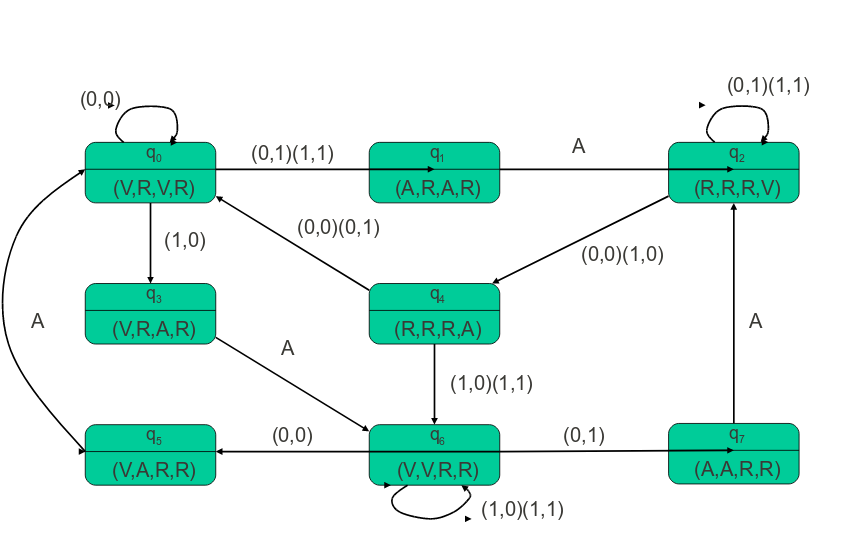
\includegraphics[width=0.7\linewidth]{3}
		\caption{}
		\label{fig:3}
	\end{figure}

	\newpage
	\section{Presentación del problema}
	\subsection{Lenguaje definido}
	\section{Diagramas de Conway}
	\section{EBNF}
	\section{Tablas de Tokens}
	\newpage
	\section{¿Cómo se va a construir el procesador del lenguaje diseñado?}
	\begin{figure}[h]
		\centering
		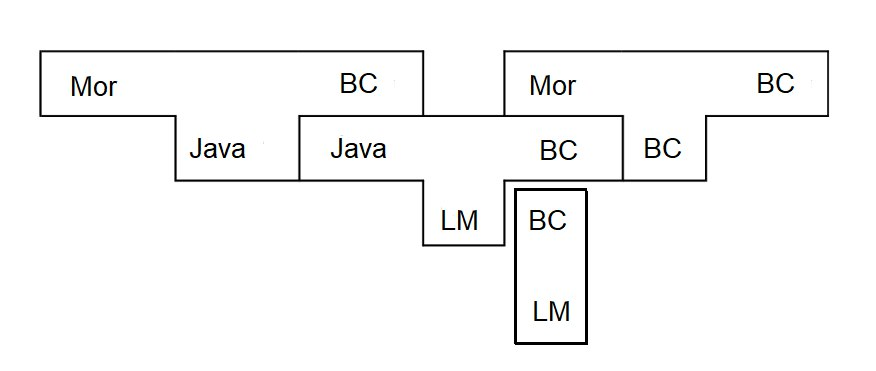
\includegraphics[width=0.7\linewidth]{5}
		\caption{}
		\label{fig:5}
	\end{figure}
	
	\newpage
	\begin{thebibliography}{99}
		\bibitem{Moore1} Autómatas de Moore
	
	\end{thebibliography}
	
	
	
	
	
\end{document}